\documentclass{llncs}

\renewcommand\floatpagefraction{.8}
\renewcommand\topfraction{.8}
\renewcommand\bottomfraction{.8}
\renewcommand\textfraction{.2}   

%\renewcommand\textfloatsep{0.3cm}
%\renewcommand\baselinestretch{0.95}
%% \addtolength{\textheight}{0.6cm}
%% \addtolength{\topmargin}{-0.25cm}
%% \addtolength{\textwidth}{0.1cm}

\usepackage{xcolor}
\usepackage{listings}
\usepackage{amsmath}
\usepackage{amssymb}
\usepackage{calc}
\usepackage{rotating}
\usepackage{subfigure}
\usepackage[ruled,vlined,linesnumbered]{algorithm2e}

\usepackage{pgf}
\usepackage{tikz}

% \usepackage{electComp}
\usetikzlibrary{decorations,decorations.pathmorphing,decorations.pathreplacing}
\usetikzlibrary{arrows,automata}
\usetikzlibrary{positioning}

% \tikzstyle{loop above}=[in=75,out=105,loop]

\tikzset{
    state/.style={
      rectangle,
      rounded corners,
      draw=black, very thick,
      minimum height=2em,
      inner sep=2pt,
      text centered,
    },
}

\tikzset{
    location/.style={
      circle,
      minimum size=15pt,
      draw=black,
      text=black,
      inner sep=1.5pt
    },
}

\newcommand{\todo}[1]{{\bf \textcolor{red}{[#1]}}}

%% \newtheorem{definition}{Definition}[section]

\newcommand{\IM}{\ensuremath{\mathit{IM}}}
\newcommand{\BC}{\ensuremath{\mathit{BC}}}
\newcommand{\A}{\ensuremath{\mathcal{A}}}

\newcommand{\Reals}{\ensuremath{\mathbb{R}}}
\newcommand{\Naturals}{\ensuremath{\mathbb{N}}}
\newcommand{\Ints}{\ensuremath{\mathbb{Z}}}

% Booleens
\newcommand{\false}{{\tt false}}
\newcommand{\true}{{\tt true}}

\newcommand{\trans}[1]{\ensuremath{\overset{#1}{\rightarrow}}}
\newcommand{\Trans}[1]{\ensuremath{\overset{#1}{\Rightarrow}}}
\newcommand{\project}[1]{\ensuremath{\downarrow_{#1}}}
\newcommand{\telapse}{\ensuremath{\uparrow}}
\newcommand{\elapse}{\ensuremath{\nearrow}}
\newcommand{\valuation}{\ensuremath{\mathcal{V}}}

%% \newcommand{\qed}{\ensuremath{\square}}

\lstdefinelanguage{pha}
{
morekeywords=[1]{automaton, contr_var, synclabs, loc, while, wait, when, sync, do, goto, end, initially},
alsoletter={=},
morekeywords=[2]{==,=},
keywordstyle=[2]{\tt},
sensitive,
morecomment=[l]{//},
morecomment=[s]{/*}{*/},
morestring=[b]",
escapeinside={/*@}{@*/},
basicstyle=\sffamily\footnotesize,
breaklines=true,
xleftmargin=0.8cm,
numbers=left,
mathescape=true
}[keywords,comments,strings]

\lstdefinelanguage{imi}
{
morekeywords=[1]{automaton, var, clock, discrete, parameter, analog, synclabs, loc, while, wait, when, sync, do, goto, end, initially},
alsoletter={=},
morekeywords=[2]{==,=},
keywordstyle=[2]{\tt},
sensitive,
morecomment=[l]{//},
morecomment=[s]{/*}{*/},
morestring=[b]",
escapeinside={(@}{@)},
basicstyle=\sffamily\footnotesize,
breaklines=true,
xleftmargin=0.8cm,
numbers=left,
mathescape=true
}[keywords,comments,strings]


%%%%%%%%%%%%%%%%%%%%%%%%%%%%%%%%%%%%%%%%%%%%%%%%%%%%%%%%%%%
%%%%%%%%%%%%%%%%%%%%%%%%%%%%%%%%%%%%%%%%%%%%%%%%%%%%%%%%%%%
\begin{document}

\title{Parametric Verification and Test Coverage for Hybrid Automata
  Using the Inverse Method}

\author{Laurent Fribourg \and Ulrich K\"uhne}

\institute{LSV ENS de Cachan, 94235 Cachan, France \\
  \email{\{kuehne,fribourg\}@lsv.ens-cachan.fr}
}


\maketitle

\begin{abstract}
  Hybrid systems combine continuous and discrete behavior.  Hybrid
  Automata are a powerful formalism for the modeling and verification
  of such systems. A common problem in hybrid system verification is
  the good parameters problem, which consists in identifying a set of
  parameter valuations which guarantee a certain behavior of a
  system. Recently, a method has been presented for attacking this
  problem for Timed Automata. In this paper, we show the extension of
  this methodology for hybrid automata with linear and affine
  dynamics. The method is demonstrated with a hybrid system benchmark
  from the literature.
\end{abstract}


%%%%%%%%%%%%%%%%%%%%%%%%%%%%%%%%%%%%%%%%%%%%%%%%%%%%%%%%%%%%%%%%%%%%%%%%%%%%
\section{Introduction} \label{sec:intro}
%% 
%% - definition hybrid systems
%% - models of hybrid systems
%% - verification problems
%% - good parameter problem
%% - inverse method
%% - cartography
%% - applications

Hybrid systems combine continuous and discrete behavior. They are
especially useful for the verification of embedded systems, as they
allow the unified modeling and the interaction of discrete control and
the continuous environment or system state such as position,
temperature or pressure. 

There are several classes of formal models for hybrid systems. In
general, there is a trade-off between the expressivity of the model
and the complexity of the algorithmic apparatus that is needed for its
formal analysis. Linear Hybrid Automata (LHA) provide a good
compromise. In contrast to more general hybrid automata models, which
allow arbitrary dynamics of the continuous state variables, LHA are
restricted to linear dynamics. This allows the use of efficient
algorithms based on convex polyhedra. Furthermore, more complex
dynamics -- like hybrid automata with affine dynamics (AHA) -- can
easily be approximated conservatively by LHA.  Although reachability
is undecidable for LHA \cite{HKPV:95}, practically relevant results
have been obtained using this formalism \cite{HHW:97}.
%\cite{SMF:97,Fre:2006}.

For the modeling of embedded systems it is handy to use
\emph{parameters} either to describe uncertainties or to introduce
tuning parameters that are subject to optimization. Instead of setting
these parameters manually and then verifying the resulting concrete
system, parameterized models are used to perform automatic
\emph{parameter synthesis}. A common assumption is the existence of a
set of bad states that should never be reached. Then the parameter
synthesis can be solved by treating the parameters as additional state
variables and computing the reachable states of the parameterized
system in a standard manner\cite{HHW:97}. However, this standard
approach is not feasible except for very simple cases. It is therefore
essential to dynamically prune the search space. The method presented
in \cite{FJK:2008} is based on the CEGAR
approach, iteratively refining a constraint over the parameters by
discarding states that violate a given property. A similar refinement scheme
has already been used for (non-parameterized) reachability problems of hybrid
systems (see e.g.~\cite{JKWC:2007}), starting with an abstraction and refining until the property has been
proved or a counterexample has been found.

While these traditional approaches to parameter synthesis are based on
the analysis of bad states or failure traces, a complementary -- or
\emph{inverse} -- method has been proposed in \cite{ACEF:2009}. It
uses a parameter instantiation that is known to guarantee a
\emph{good} behavior in order to derive a constraint on the parameters
that leads to the same behavior. While the algorithm in
\cite{ACEF:2009} is restricted to Timed Automata (TA), we present its
extension to LHA in this paper. 

There are different scenarios for the application of the presented
approach. If a given parameter instantiation is known to guarantee
certain properties, the inverse method can be used to derive an
enlarged area of the parameter space that preserves these properties,
while possibly allowing for enhanced performance of the system. 
In the
%same time, the \emph{robustness} of the parameter choice can be
%proven. Since real world systems are often subject to uncertainties
%wrt.~to environment conditions, it is not advisable to choose a
%parameter instantiation that lies on the very edge to
%malfunction. Finally, it can be used if the parameterized
%\emph{verification} of a safety property is not feasible. In this
%case, a pointwise verification for a set of parameter instantiations
%is performed. 
The inverse method can %then 
also be used to obtain a measure
of \emph{coverage} of the parameter space by computing the zones of
equivalent behavior for each point. This approach is also known as
\emph{behavioral cartography} \cite{AF:2010} and will be discussed in
this paper. While the natural extension of these algorithms works well
for simple LHA, it does not scale well to LHA models that approximate
more complex dynamics. Therefore, we present an enhanced algorithm
that can be applied on affine hybrid automata.

The presented algorithms are implemented in a tool called IMITATOR
(\emph{Inverse Method for Inferring Time AbstracT behaviOR})
\cite{And:2010}. The tool has originally been developed for the
analysis of TA. The new version IMITATOR~3 implements the semantics of
LHA as presented in Sect.~\ref{sec:lha}. The manipulation of
symbolic states is based on the polyhedral operations of the Parma
Polyhedra Library~\cite{BHZ:2009}.

%The paper is structured as follows. First, we will discuss related
%work in Sect.~\ref{sec:related}. In Sect.~\ref{sec:lha}, the formal
%basis for the rest of the paper is given. The algorithms are
%introduced and discussed in Sect.~\ref{sec:algo}. 
%The results are discussed in
%Sect.~\ref{sec:disc} 
%The paper is concluded in
%Sect.~\ref{sec:concl}. 
Throughout the paper, we will use a running
example -- a distributed temperature control system -- to illustrate
the presented concepts. Further examples can be found in \cite{FK:2011}.

%%%%%%%%%%%%%%%%%%%%%%%%%%%%%%%%%%%%%%%%%%%%%%%%%%%%%%%%%%%%%%%%%%%%%%%%%%%%
\section{Related Work} \label{sec:related}

The presented approach exhibits the same general differences with the
CEGAR-based approach of \cite{FJK:2008} at the LHA level as formerly
at the TA level. First, the input of CEGAR-based methods is a bad
location to be avoided while the input of our inverse method is a
good reference valuation for the parameters; second, the constraint in
CEGAR-based methods guarantees the avoidance of bad locations while the
constraint generated by the inverse method guarantees the same behavior
(in terms of discrete moves) as under the reference valuation.

Additionally, our inverse method based approach for LHA is comparable
to the symbolic analysis presented in \cite{AKRS:2008} for improving
the simulation coverage of hybrid systems.  In their work, Alur et
al.~start from an initial state $x$ and a discrete-time simulation
trajectory, and compute a constraint describing those initial states
that are guaranteed to be equivalent to $x$, where two initial states
are considered to be equivalent if the resulting trajectories contain
the same locations at each discrete step of execution.  The same kind
of constraint can be generated by our inverse method when initial
values of the continuous variables are defined using parameters. The
two methods are however methodologically different.  On the one hand,
the generalization process done by the inverse method works, using
forward analysis, by refining the current constraint over the
parameters that repeatedly discards the generated states that are
incompatible with the initial valuation of $x$; on the other hand, the
method of Alur et al.~generalizes the initial value of $x$ by
performing a backward propagation of sets of equivalent states. This
latter approach can be practically done because the system is supposed
to be {\em deterministic}, thus making easy the identification of
transitions between discrete states during the execution. Our inverse
method, in contrast, can also treat nondeterministic systems.

The approach presented in \cite{JFG+:2007} shares a similar goal,
namely identifying for single test cases a robust environment that
leads to the same qualitative behavior. Instead of using symbolic
reachability techniques, their approach is based on the stability of
the continuous dynamics. By using a bisimulation function (or
contraction map), a robust neighborhood can be constructed for each
test point. As traditional numeric simulation can be used, this makes
the technique computationally effective. But, for weakly stable
systems, a lot of test points have to be considered in order to
achieve a reasonable coverage. For some of the examples in
\cite{JFG+:2007}, we achieve better or comparable results
(see \cite{FK:2011}).

%Note that both \cite{AKRS:2008} and \cite{JFG+:2007} only consider the
%coverage of the initial states, while our approach can be applied in the
%more general context of parameter synthesis.



%%%%%%%%%%%%%%%%%%%%%%%%%%%%%%%%%%%%%%%%%%%%%%%%%%%%%%%%%%%%%%%%%%%%%%%%%%%%
\section{Hybrid Automata with Parameters} \label{sec:lha}
\subsection{Basic Definitions}
In the sequel, we will refer to a set of continuous variables $X =
{x_1, \dots, x_N}$ and a set of parameters $P = {p_1, \dots, p_M}$. 
Continuous variables can take any real value. We define a valuation as
a function $w: X \rightarrow \Reals$, and the set of valuations
over variables $X$ is denoted by $\valuation(X)$. A valuation $w$ will
often be identified with the point $(w(x_1), \dots, w(x_N)) \in
\Reals^N$. A parameter valuation is a function $\pi: P \rightarrow
\Reals$ mapping the parameters to the  real numbers.

Given a set of variables $X$, a linear inequality has the form $\sum
_{i=1}^{N} \alpha_i x_i \bowtie \beta,$ where $x_i \in X$,
$\alpha_i, \beta \in \Ints$ and $\bowtie\; \in \{<, \leq, =\}$. A
convex linear constraint is a finite conjunction of linear
inequalities. The set of convex linear constraints over $X$ is denoted
by $\mathcal{L}(X)$. For a constraint $C \in \mathcal{L}(X)$ satisfied
by a valuation $w \in \mathcal{V}(X)$, we write $w \models C$. For a
constraint over continuous variables and parameters $C \in
\mathcal{L}(X \cup P)$ satisfied by a valuation $w$ and a parameter
valuation $\pi$, we write $\left<w, \pi\right> \models C$. By
convention, we also write $w \models C$ for partial valuations. For
example, a valuation $w \in \mathcal{V}(X)$ is said to satisfy a
constraint $C \in \mathcal{L}(X \cup P)$ iff it can be extended with
at least one parameter valuation $\pi$ such that $\left<w, \pi\right>
\models C$.

Sometimes we will refer to a variable domain $X'$, which is obtained
by renaming the variables in $X$. Explicit renaming of variables is
denoted by the substitution operation. Here, $(C)_{[X/Y]}$ denotes the
constraint obtained by replacing in $C$ the variables of $X$ by the variables
of $Y$.

A convex linear constraint can also be interpreted as a set of points
in the space $\Reals^N$, more precisely as a convex polyhedron. We
will use these notions synonymously. In this geometric context, a
valuation satisfying a constraint is equivalent to the polyhedron
containing the corresponding point, written as $w \in C$. Also here,
for a partial valuation $w$ (i.e.~a point of a subspace of $C$), we
write $w \in C$ iff $w$ is contained in the projection of $C$ on the
variables of $w$. 

\begin{definition}\label{def:lha}
  Given a set of continuous variables $X$ and a set of parameters $P$,
  a {\em (parameterized) hybrid automaton} is a tuple $\A = (\Sigma, Q, q_0,
  I, D, \rightarrow)$, consisting of the following
  \begin{itemize}
    \item a finite set of actions $\Sigma$
    \item a finite set of locations $Q$
    \item an initial location $q_0 \in Q$ %% , where $K \subseteq I_{q_0}$
    \item a convex linear invariant $I_q \in \mathcal{L}(X \cup P)$ for each
      location $q$
    \item an activity $D_q : \Reals^n \rightarrow \Reals^n$ for each
      location $q$ 
    \item discrete transitions $q \xrightarrow{g, a, \mu} q'$, with
      guard condition $g \in \mathcal{L}(X \cup P)$, action $a \in \Sigma$
      and a jump relation $\mu \in \mathcal{L}(X \cup P \cup X')$.
  \end{itemize}
  Given a parameter constraint $K \in \mathcal{L}(P)$, the automaton
  $\A$ with the parameters restricted to $K$ is denoted by
  $\A(K)$. Given a parameter valuation $\pi$, the automaton $\A$ with
  all parameters instantiated as in $\pi$ is denoted by $\A[\pi]$.
\end{definition}

Without loss of generality,
it is assumed here that all continuous variables $x$ are initialized
with $x=0$. Arbitrary initial values can be modeled by adding a
transition with appropriate variable updates.
Parameters can be seen as additional state variables which do
not evolve in time (null activity).

The activities $D_q$ describe how the continuous variables evolve
within each location $q$. In order to obtain automata models which can
be symbolically analyzed, restrictions have to be made to these
activities. This leads to the following classes of hybrid automata.

\begin{definition}
  We define the following subclasses of hybrid automata.

  \begin{itemize}
  \item[(1)] A \emph{linear hybrid automaton} (LHA) is a hybrid automaton,
    where in each location $q$, the activity is given by a convex
    linear constraint $D_q \in \mathcal{L}(\dot{X})$ over the time
    derivatives of the variables.

  \item[(2)] An \emph{affine hybrid automaton} (AHA) is a hybrid
    automaton, where in each location $q$, the activity is given by a
    convex linear constraint $D_q \in \mathcal{L}(X \cup \dot{X})$
    over the variables and the time derivatives.
  \end{itemize}
\end{definition}

The class of timed automata can be obtained by restricting the
derivatives to $\dot{x} = 1$ and limiting the jump relations to either
$x' = x$ or $x' = 0$ (clock reset) for all variables $x \in X$. In
total, the automata models defined above form a hierarchy $TA \subset
LHA \subset AHA$.

The reachable states of LHA can be efficiently represented by convex
polyhedra. Due to the more complex dynamics, this is not true for
AHA. In the following, we consider linear hybrid automata with
parameters. But, AHA can be approximated by LHA with arbitrary
precision by partitioning the state space, as e.g.~described
in~\cite{Fre:2008}. In Sect.~\ref{sec:laha} it is discussed, how
these techniques can be adapted to suit our methods. In the following,
we give an example of a hybrid system, that will later on be used to
illustrate the approaches proposed here. 

% \begin{example}
%   The \emph{Fischer protocol} provides mutual exclusion for a
%   distributed system with skewed clocks. The processes communicate via
%   a shared variable $k$. Before entering a critical section, each
%   process reads the variable $k$. If $k$, then the process sets $k$ to
%   its own unique ID, which takes at most $a$ time units. If, after
%   waiting for $b$ time units, $k$ is still set to its own ID, the
%   process is allowed to enter the critical section. Otherwise, the
%   access cycle starts again. After leaving the critical section, $k$
%   is reset to zero. \figurename~\ref{fig:fischer} shows an
%   instantiation of the Fischer protocol for two processes, where $P_1$
%   has a relative clock speed between $\frac{4}{5}$ and $1$, and $P_2$
%   has a relative clock speed between $1$ and $\frac{11}{10}$.

% \begin{figure}[tb]
%   \centering
%   \footnotesize
%   \begin{tikzpicture}[->,>=stealth']

%     \begin{scope}
%     \node[state] (Q1)
%     {
%       \begin{tabular}{c}
%         $Q_1$ \\
%         \hline \\[-1em]
%         \begin{tabular}{l}
%           $\dot{x} \in [\frac{4}{5},1]$ \\
%         \end{tabular}
%       \end{tabular}
%     };
    
%     \node[state,
%     below of=Q1,
%     node distance=2.5cm] (Q2)
%     {
%       \begin{tabular}{c}
%         $Q_2$ \\
%         \hline \\[-1em]
%         \begin{tabular}{l}
%           $\dot{x} \in [\frac{4}{5},1]$ \\
%           $x \leq a$ 
%         \end{tabular}
%       \end{tabular}
%     };

%     \node[state,
%     below of=Q2,
%     node distance=2.5cm] (Q3)
%     {
%       \begin{tabular}{c}
%         $Q_3$ \\
%         \hline \\[-1em]
%         \begin{tabular}{l}
%           $\dot{x} \in [\frac{4}{5},1]$ \\
%         \end{tabular}
%       \end{tabular}
%     };

%     \node[state,
%     below of=Q3,
%     node distance=2cm] (CS)
%     {
%       \begin{tabular}{c}
%         critical \\
%         \hline \\[-1em]
%         \begin{tabular}{l}
%           $\dot{x} \in [\frac{4}{5},1]$ \\
%         \end{tabular}
%       \end{tabular}
%     };

%     \node[left of=Q1, node distance=2 cm] (INIT) {
%       $k = 0$
%     };

%     \path
%     (INIT) edge (Q1)

%     (Q1)  edge node[anchor=left,right]
%     {
%       \begin{tabular}{l}
%         $k = 0 /$ \\
%         $x' = 0$
%       \end{tabular}
%     } (Q2)
    
%     (Q2) edge node[anchor=left,right]
%     {
%       \begin{tabular}{l}
%         $true /$ \\
%         $k' = 1,$\\
%         $x' = 0$
%       \end{tabular}
%     } (Q3)

%     (Q3)  edge[bend left=45] node[anchor=right,left]
%     {
%       \begin{tabular}{r}
%         $x \geq b \wedge$\\
%         $k \neq 1$ \\
%       \end{tabular}
%     } (Q1)

%     (Q3)  edge node[anchor=right,left]
%     {
%       \begin{tabular}{r}
%         $x \geq b \wedge k = 1$ \\
%       \end{tabular}
%     } (CS)

%     (CS)  edge[bend right=50] node[anchor=left,right]
%     {
%       \begin{tabular}{l}
%         $true /$\\
%         $k' = 0$
%       \end{tabular}
%     } (Q1);
%   \end{scope}

%   \begin{scope}[xshift=6cm]
%     \node[state] (Q1)
%     {
%       \begin{tabular}{c}
%         $Q_1$ \\
%         \hline \\[-1em]
%         \begin{tabular}{l}
%           $\dot{y} \in [1,\frac{11}{10}]$ \\
%         \end{tabular}
%       \end{tabular}
%     };
    
%     \node[state,
%     below of=Q1,
%     node distance=2.5cm] (Q2)
%     {
%       \begin{tabular}{c}
%         $Q_2$ \\
%         \hline \\[-1em]
%         \begin{tabular}{l}
%           $\dot{y} \in [1,\frac{11}{10}]$ \\
%           $y \leq a$ 
%         \end{tabular}
%       \end{tabular}
%     };

%     \node[state,
%     below of=Q2,
%     node distance=2.5cm] (Q3)
%     {
%       \begin{tabular}{c}
%         $Q_3$ \\
%         \hline \\[-1em]
%         \begin{tabular}{l}
%           $\dot{y} \in [1,\frac{11}{10}]$ \\
%         \end{tabular}
%       \end{tabular}
%     };

%     \node[state,
%     below of=Q3,
%     node distance=2cm] (CS)
%     {
%       \begin{tabular}{c}
%         critical \\
%         \hline \\[-1em]
%         \begin{tabular}{l}
%           $\dot{y} \in [1,\frac{11}{10}]$ \\
%         \end{tabular}
%       \end{tabular}
%     };

%     \node[left of=Q1, node distance=2 cm] (INIT) {
%       $k = 0$
%     };

%     \path
%     (INIT) edge (Q1)

%     (Q1)  edge node[anchor=left,right]
%     {
%       \begin{tabular}{l}
%         $k = 0 /$ \\
%         $y' = 0$
%       \end{tabular}
%     } (Q2)
    
%     (Q2) edge node[anchor=left,right]
%     {
%       \begin{tabular}{l}
%         $true /$ \\
%         $k' = 2,$\\
%         $y' = 0$
%       \end{tabular}
%     } (Q3)

%     (Q3)  edge[bend left=45] node[anchor=right,left]
%     {
%       \begin{tabular}{r}
%         $y \geq b \wedge$\\
%         $k \neq 2$ \\
%       \end{tabular}
%     } (Q1)

%     (Q3)  edge node[anchor=right,left]
%     {
%       \begin{tabular}{r}
%         $y \geq b \wedge k = 2$ \\
%       \end{tabular}
%     } (CS)

%     (CS)  edge[bend right=50] node[anchor=left,right]
%     {
%       \begin{tabular}{l}
%         $true /$\\
%         $k' = 0$
%       \end{tabular}
%     } (Q1);
%   \end{scope}

%   \end{tikzpicture}
%   \caption{Fischer mutual exclusion protocol}\label{fig:fischer}
% \end{figure}
% \end{example}


\begin{example} \label{ex:rhb}
The \emph{room heating benchmark} (RHB) has been described in
\cite{FI:2004}. It models a distributed temperature control
system. There are $m$ movable heaters for $n > m$ rooms. The
temperature $x_i$ in each room $i$ is a continuous variable that
depends on the (constant) outside temperature $u$, the temperature of
the adjacent rooms, and whether there is an activated heater in the
room.

Depending on the relations between the temperatures measured,
the heaters will be moved. If there is no heater in room $i$, a heater
will be moved there from an adjacent room $j$, if the temperature has
reached a threshold $x_i \leq get_i$ and there is a minimum difference
of the temperatures $x_j - x_i \geq dif_i$.  Note that in contrast
with the RHB modeled in \cite{AKRS:2008}, the heater move from a room
to another one is nondeterministic, since multiple guard conditions
can be enabled simultaneously (in \cite{AKRS:2008}, the nondeterminism
is resolved by moving only the heater with the smallest index).
%
The dynamics is given by equations of the form:
\begin{equation}\label{eq:rhb}
  \dot{x}_i = c_i h_i + b_i (u - x_i) + \sum \limits_{i\neq j} a_{i,j}(x_j - x_i)
\end{equation}
where $a_{i,j}$ are constant components of a symmetric adjacency
matrix, constants $b_i$ and $c_i$ define the influence of the outside
temperature and the effectiveness of the heater for each room $i$, and
$h_i = 1$ if there is a heater in room $i$ and $h_i = 0$ otherwise.
%
Here, we will study an instantiation of RHB as given in
\cite{AKRS:2008} with $n=3, m=2$, outside temperature $u=4$, the
constants $b = (0.4, 0.3, 0.4), c = (6,7,8)$. The adjacency matrix
$a_{i,j}$ is given as $\left(\begin{smallmatrix}
      0.0 \;\; & 0.5 & \;\; 0.0 \\
      0.5 \;\; & 0.0 & \;\; 0.5 \\
      0.0 \;\; & 0.5 & \;\; 0.0 \\
\end{smallmatrix}\right)$
and the thresholds are set to $get = 18$ and $dif = 1$ for all rooms.

\begin{figure}[tb]
  \centering
  \footnotesize
  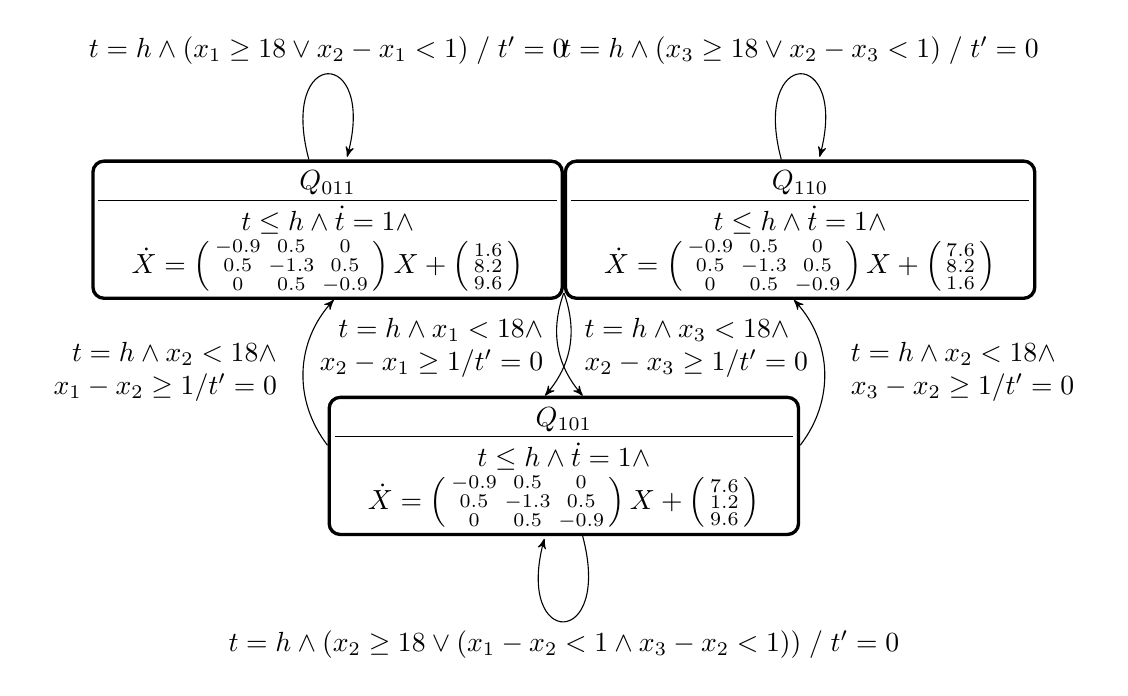
\begin{tikzpicture}[->,>=stealth']

    \node[state] (Q011) at (0,3)
    {
      \begin{tabular}{c}
        $Q_{011}$ \\
        \hline \\[-1em]
        \begin{tabular}{c}
          $t \leq h \wedge \dot{t} = 1 \wedge$ \\
          $\dot{X} = \left(\begin{smallmatrix}
              -0.9 & 0.5 & 0 \\
              0.5 & -1.3 & 0.5 \\
              0 & 0.5 & -0.9
          \end{smallmatrix} \right) X + \left(\begin{smallmatrix}
            1.6 \\ 8.2 \\ 9.6
          \end{smallmatrix}\right)$ \\
        \end{tabular}
      \end{tabular}
    };
    
    \node[state] (Q101) at (3,0)
    {
      \begin{tabular}{c}
        $Q_{101}$ \\
        \hline \\[-1em]
        \begin{tabular}{c}
          $t \leq h \wedge \dot{t} = 1 \wedge$ \\
          $\dot{X} = \left(\begin{smallmatrix}
              -0.9 & 0.5 & 0 \\
              0.5 & -1.3 & 0.5 \\
              0 & 0.5 & -0.9
            \end{smallmatrix} \right) X + \left(\begin{smallmatrix}
              7.6 \\ 1.2 \\ 9.6
            \end{smallmatrix}\right)$ \\
        \end{tabular}
      \end{tabular}
    };

    \node[state] (Q110) at (6,3)
    {
      \begin{tabular}{c}
        $Q_{110}$ \\
        \hline \\[-1em]
        \begin{tabular}{c}
          $t \leq h \wedge \dot{t} = 1 \wedge$ \\
          $\dot{X} = \left(\begin{smallmatrix}
              -0.9 & 0.5 & 0 \\
              0.5 & -1.3 & 0.5 \\
              0 & 0.5 & -0.9 
            \end{smallmatrix} \right) X + \left(\begin{smallmatrix}
              7.6 \\ 8.2 \\ 1.6
            \end{smallmatrix}\right)$ \\
        \end{tabular}
      \end{tabular}
    };

    \path

    (Q011) edge[loop above] node{$t=h \wedge (x_1 \geq 18 \vee x_2-x_1 < 1) \; / \; t' = 0$} (Q011)

    (Q110) edge[loop above] node{$t=h \wedge (x_3 \geq 18 \vee x_2-x_3 < 1) \; / \; t' = 0$} (Q110)

    (Q101) edge[loop below] node{$t=h \wedge (x_2 \geq 18 \vee (x_1-x_2 < 1 \wedge x_3-x_2 < 1))\; / \; t' = 0$} (Q101)

    (Q011)  edge[bend left=30] node[anchor=right,left]
    {
      \begin{tabular}{r}
        $t = h \wedge x_1 < 18 \wedge$ \\
        $x_2 - x_1 \geq 1 / t' = 0$
      \end{tabular}
    } (Q101)

    (Q101)  edge[bend left=40] node[anchor=right,left]
    {
      \begin{tabular}{r}
        $t = h \wedge x_2 < 18 \wedge$ \\
        $x_1 - x_2 \geq 1 / t' = 0$
      \end{tabular}
    } (Q011)

    (Q110)  edge[bend right=30] node[anchor=left,right]
    {
      \begin{tabular}{l}
        $t = h \wedge x_3 < 18 \wedge$ \\
        $x_2 - x_3 \geq 1 / t' = 0$
      \end{tabular}
    } (Q101)

    (Q101)  edge[bend right=40] node[anchor=left,right]
    {
      \begin{tabular}{l}
        $t = h \wedge x_2 < 18 \wedge$ \\
        $x_3 - x_2 \geq 1 / t' = 0$
      \end{tabular}
    } (Q110)
    
    ;
  \end{tikzpicture}
  \caption{Automaton model for room heating benchmark}\label{fig:rhbaut}
\end{figure}
%
The system can be modeled as an AHA, as shown in
\figurename~\ref{fig:rhbaut}. There are three control modes, corresponding
to the positions of the two heaters. The automaton has four variables,
the temperatures $X = \{x_1, x_2, x_3\}$ and a variable $t$ acting as
clock. In this example, the temperatures are sampled at a constant
rate $\frac{1}{h}$, where $h$ is a parameter of the automaton.  This
sampling scheme is used in the models of sampled-data hybrid systems
of \cite{SK:2000} and simulink/stateflow models \cite{AKRS:2008}. 

% Since the invariants associated to these modes have a disjunctive form
% (the threshold $get$ is not reached \emph{or} the difference $dif$ is
% not reached yet), they have to be modeled by multiple locations with
% convex invariants. This leads to a total of eleven locations.
\end{example}


%%%%%%%%%%%%%%%%%%%%%%%%%%%%%%%%%%%%%%%%%%%%%%%%%%%%%%%%%%%%%%%%%%%%%%%%%%%%
\subsection{Symbolic semantics}
The symbolic semantics of a LHA $\A(K)$ are defined at the level of
constraints, a symbolic state is a pair $(q,C)$ of a location $q$ and
a constraint $C$ over variables and parameters. The corresponding
operations are therefore performed on convex polyhedra rather than on
concrete valuations. One necessary operation is the progress of time
within a symbolic state, modeled by the \emph{time-elapse} operation.

\begin{definition}\label{def:telapse}
Given a symbolic state $(q,C)$, the states reached by letting $t$ time
units elapse, while respecting the invariant of $q$, are characterized
as follows:
\begin{equation*}
 w' \in C \telapse_{q}^{t} \quad \text{iff} \quad \exists w \in C, v \in D_q: w' = w + t\cdot v \wedge w' \in I_q. 
\end{equation*}
We write  $w' \in C \telapse_{q} $ if $ w' \in C \telapse_{q}^{t}$
for some $t \in \Reals_+$.
\end{definition}

Note that due to the convexity of the invariants, if $C \subseteq I_q$
and $C\telapse_{q}^{t} \subseteq I_q$, then also $\forall t' \in
[0,t]: C\telapse_{q}^{t'} \subseteq I_q$. The operator preserves the
convexity of $C$.
Furthermore, the operator $C \project{X}$ denotes the projection of the
constraint $C$ on the variables in $X$. Based on these definitions, the
symbolic semantics of a LHA $\A(K)$ is given by a labeled transition
system (LTS).

\begin{definition}\label{def:lts}
  A labeled transition system over a set of symbols $\Sigma$ is a
  triple $(S, S_0, \Rightarrow)$ with a set of states $S$, a set
  of initial states $S_0 \subseteq S$ and a transition relation
  $\Rightarrow \; \subseteq S \times \Sigma \times S$. We write $s
  \Trans{a} s'$ for $(s, a, s') \in \Rightarrow$. A run of length $m$
  is a finite alternating sequence of states and symbols of the form
  $s_0 \Trans{a_0} s_1 \Trans{a_1} \dots \Trans{a_{m-1}} s_m$, where
  $s_0 \in S_0$. 
%A state $s_m$ is reachable if it is the last state of some run $R$.
\end{definition}

\begin{definition}\label{def:ssem}
  The symbolic semantics of LHA $\A(K)$ is a LTS with
  \begin{itemize}
  \item states $S = \{ (q,C) \in Q \times \mathcal{L}(X \cup P) \mid C \subseteq I_q \}$
  \item initial state $s_0 = (q_0, C_0)$ with $C_0 =  K \wedge [\bigwedge_{i=1}^N x_i=0] \telapse_{q_0}$
  \item discrete transitions $(q,C) \trans{a} (q',C')$ if exists $q \trans{a,g,\mu} q'$ and \\
    $C' = \big( \left[ C(X) \wedge g(X) \wedge \mu(X,X') \right]
    \project{X'} \wedge I_{q'}(X') \big)_{[X'/X]}$
  \item delay transitions $(q,C) \trans{t} (q,C')$ with $C' = C \telapse_q^t$
  \item transitions $(q,C) \overset{a}{\Rightarrow} (q',C')$ if $\exists t,C'': (q,C) \trans{a} (q',C'') \trans{t} (q',C')$ %, or as a closed formula:\\  $C' = \big( \left[ \left[ C(X) \wedge g(X) \wedge \mu(X,X') \right] \project{X'} \wedge I_{q'}(X') \right] \telapse_{q'} \big)_{[X'/X]}$
  \end{itemize}
\end{definition}

The {\em trace of a symbolic run} $(q_0, C_0) \Trans{a_0} \dots
\Trans{a_{m-1}} (q_m, C_m)$ is obtained by projecting the symbolic
states to the locations, which gives: $q_0 \Trans{a_0} \dots
\Trans{a_{m-1}} q_m$. Two runs are said to be {\em equivalent}, if
their corresponding traces are equal.

The set of states reachable from any state in a set $S$ in exactly $i$
steps is denoted as $Post^{i}_{\A(K)}(S) = \{s' \mid \exists s \in S: s \Trans{a_{0}} \dots
\Trans{a_{i-1}} s'\}$. Likewise, the set of all reachable states from
$S$ is defined as $Post^{*}_{\A(K)}(S) = \bigcup_{i\geq
  0}Post^{i}_{\A(K)}$. The reachable states of an automaton $\A(K)$
are defined as $Reach_{\A(K)} = Post^{*}_{\A(K)}(\{s_0\})$, where
$s_0$ is the initial state of $\A(K)$.

Note that during a run of $\A(K)$, the parameter
constraints associated to the reachable states can only get stronger,
since the parameters do not evolve under the time elapse operation,
and can only be further constrained by invariants or guard
conditions. This gives rise to the following observation.

\begin{lemma}\label{lem:narrow}
  For any reachable state $(q,C) \in Reach_{\A(K)}$, it holds that
  $(\exists X: C) \subseteq K$. This implies that for each parameter
  valuation $\pi \models C$, also $\pi \models K$. 
\end{lemma}

The lemma follows directly from the definition of the symbolic
semantics. We say that a state $(q,C)$ is \emph{compatible} with a
parameter valuation $\pi$, or just \emph{$\pi$-compatible}, if $\pi
\models C$. Conversely, it is \emph{$\pi$-incompatible} if $\pi
\not\models C$.
%
These observations are the basis for the \emph{Inverse Method}, 
is described in next  section.

%%%%%%%%%%%%%%%%%%%%%%%%%%%%%%%%%%%%%%%%%%%%%%%%%%%%%%%%%%%%%%%%%%%%%%%%%%%%
\section{Algorithm}\label{sec:algo}
\subsection{Inverse Method}

The Inverse Method for LHA attacks the good parameters problem by
generalizing a parameter valuation $\pi$ that is known to guarantee a
good behavior. Thereby, the valuation $\pi$ is relaxed to a constraint
$K$ such that the \emph{discrete behavior} -- i.e.~the set of
traces -- of $\A[\pi]$ and $\A(K)$ is identical. The algorithm has
first been described for parametric timed automata
in~\cite{ACEF:2009}. It has been applied for the synthesis of timing
constraints for memory circuits \cite{And:2009}.

\begin{algorithm}[tb]
  \SetKwInOut{Input}{input}\SetKwInOut{Output}{output}

  \Input{Parametric linear hybrid automaton $\A$} %%  of initial state $s_0 = (q_0, K_0)$} %% FIXME: what is this for?
  \Input{Valuation $\pi$ of the parameters}
  
  \Output{Constraint $K_0$ on the parameters}
  
  \BlankLine

  $ i \leftarrow 0\,;\ \  K \leftarrow \true \,; \ \ S \leftarrow \{ s_0 \} $


  % WHILE TRUE DO
  \While{\true}{
    % WHILE INCOMPATIBLE DO
    \While{there are $\pi$-incompatible states in $S$}
    {
      Select a $\pi$-incompatible state $(q, C)$ of $S$ (i.e., s.t. $\pi \not\models C$) \label{IM:select_state} \;
		
      Select a $\pi$-incompatible inequality $J$ in $(\exists X : C)$ (i.e., s.t. $\pi \not\models J$) \label{IM:select_conjunct}\;

      $K \leftarrow K \wedge\neg J $ \;
      $S \leftarrow \bigcup^i_{j = 0} \mathit{Post}^j_{\A(K)}(\{ s_0 \})$ \; \label{IM:post_update}
    } % ENDWHILE
    % \tcp*{$S$ is $\pi$-compatible}
	
    % IF
    % \lIf{$\mathit{Post}_{\A(K)}(S) = \emptyset$}
    \lIf{$\mathit{Post}_{\A(K)}(S) \sqsubseteq S $}{\Return{$K_0 \leftarrow \bigcap_{(q, C) \in S} (\exists X :C)$}} \label{IM:terminate}

    $i \leftarrow i+1$ \;
    $S \leftarrow S \cup \mathit{Post}_{\A(K)}(S)$
%%    \tcp*{$S = \bigcup^i_{j = 0} \mathit{Post}^j_{\A(K)}(\{ s_0 \})$}
    
  } % ENDWHILE

  % RETURN
  \caption{$\IM(\A, \pi)$}\label{algo:IM}
\end{algorithm}

Algorithm~\ref{algo:IM} describes the Inverse Method for LHA. The
overall structure is similar to a reachability analysis. In the main
loop, the reachable states with increasing depth $i$ are computed. In
parallel, the constraint $K$ is derived. It is initialized with
$\true$. Each time a $\pi$-incompatible state $(q,C)$ is reached, $K$
is refined such that the incompatible state is unreachable for
$\A(K)$. If $C$ is $\pi$-incompatible, then there must be at least one
inequality $J$ in its projection on the parameters ($\exists X:C$),
which is incompatible with $\pi$. The algorithm selects one such
inequality and adds its negation $\neg J$ to the constraint
$K$. Before continuing with the search, the reachable states found so
far are updated to comply with the new constraint $K$ (line
\ref{IM:post_update}). If there are no more $\pi$-incompatible states,
then $i$ is increased and the loop continues.

The algorithm stops as soon as no new states are found (line
\ref{IM:terminate}). The output of the algorithm is then a parameter
constraint $K_0$, obtained as the intersection of the constraints
associated with the reachable states.  The resulting constraint can be
characterized as follows.

\begin{proposition}
  Suppose that the algorithm $\IM(\A, \pi_0, k)$ terminates with the
  output $K_0$. Then the following holds:
  \begin{itemize}
  \item $\pi_0 \models K_0$
  \item For all $\pi \models K_0$, $\A[\pi_0]$ and $\A[\pi]$ have the same sets of traces.
  \end{itemize}
\end{proposition}

A proof along the lines of \cite{HRSV:2002} can be found in
\cite{FK:2011}. 
%In other words, 
We obtain a (convex) constraint $K_0$
including the initial point $\pi_0$, that describes a set of parameter
valuations for which the same set of traces is observable. In
particular, if $\A[\pi_0]$ is known to avoid a set of (bad) locations
for $\pi_0$, so will $\A[\pi]$ for any $\pi \models K_0$.

%Note that the intersection in line~\ref{IM:terminate} is necessary --
%rather than just returning $K$ -- in order to guarantee the
%equivalence of the traces. Without this operation, it is possible that
%the symbolic semantics of $\A(K)$ contains additional traces caused by
%deadlocks that do not occur in $\A[\pi_0]$. For more details, refer to
%\cite{ACEF:2009}. 

The algorithm $\IM$ is not guaranteed to
terminate\footnote{Termination of such a general reachability-based
  procedure cannot be guaranteed due to undecidability of reachability
  for TA with parameters and LHA \cite{HKPV:95}}.  Note also that the
presented algorithm involves nondeterminism. In
Algorithm~\ref{algo:IM} in lines \ref{IM:select_state} and
\ref{IM:select_conjunct}, one can possibly choose among several
incompatible states and inequalities. This may lead to different --
nevertheless correct -- results. This implies in particular that the
resulting constraint $K_0$ is not maximal in general. (In order to
overcome this limitation, the \emph{behavioral cartography} method
will be proposed in  Section~\ref{ss:carto}).

% \begin{example}
%   Consider again the Fischer protocol in
%   \figurename~\ref{fig:fischer}. The correct functionality of the
%   protocol (there can be at most one process in a critical section)
%   depends on the choice of the timing parameter $b$ wrt.~to the clock
%   skew of the processes and the maximum write delay $a$.  In general,
%   a high value for $b$ will guarantee that all concurrent writes will
%   be finished before a process checks variable $k$ and eventually
%   enters the critical section. For the given instantiation, it can be
%   verified that for a maximum write delay set to the unit value $a=1$,
%   the choice of $b=2$ is sufficient to guarantee a correct
%   behavior. This is however not an optimal solution.

%   Using the inverse method with the above parameter valuation $\pi_0 =
%   (1,2)$, the constraint $a \geq 0 \; \wedge \; b > \frac{11}{8}
%   a$ is generated, guaranteeing the mutual exclusion property.
%   This means that for $a=1$, it is sufficient to choose a value for
%   $b$ which is greater than $1.375$.
% \end{example}

\begin{example} \label{ex:rhb2}
  In order to enable the application of the inverse method as
  described above to the RHB from example \ref{ex:rhb}, the AHA
  automaton is converted to a LHA.  This is done using the 
%{\em    phase-portrait} approximation 
method described in \cite{Fre:2008}. 
%\cite{HW:96}. 
The space
  is partitioned into regions, and within each region, the activity
  field is overapproximated using linear sets of activity vectors.
  For each region $R$ delimiting a portion of the partitioned state
  space, the activities are statically overapproximated as
  \begin{equation*}
   \dot{x}_i \in \left[ min \{f_i(x) \mid x \in R \}, max \{f_i(x) \mid x \in R \} \right],
 \end{equation*}
  where $f_i(x)$ corresponds to the right-hand side in \eqref{eq:rhb}.
  The approximation can be made arbitrarily accurate by approximating
  over suitably small regions of the state space. Here, each region
  $R$ corresponds to a unit cube (of size 1 degree Celsius) in the
  dimensions $x_1,x_2,x_3$.

  \begin{figure}[tb]
  \centering
  \subfigure[Starting from a single point]{
    \includegraphics[width=3.5cm]{images/point_x1} \; 
    \includegraphics[width=3.5cm]{images/point_x2} \;
    \includegraphics[width=3.5cm]{images/point_x3}
    \label{fig:plot_point}
  }
  \subfigure[Starting from a tile synthesized by the Inverse Method]{
    \includegraphics[width=3.5cm]{images/plot_t_x1} \; 
    \includegraphics[width=3.5cm]{images/plot_t_x2} \;
    \includegraphics[width=3.5cm]{images/plot_t_x3}
    \label{fig:plot_zone}
  } 
  \caption{Reachable states for room heating benchmark}\label{fig:plot_rhb}
\end{figure}

%  Since the inverse method considers only the discrete behavior of a
%  system, it is well-suited for qualitative properties that
%  address the switching of discrete states, as those
%  considered in \cite{FI:2004}:
%  \begin{itemize}
%  \item All rooms eventually get a heater
%  \item In all rooms there will eventually be no heater
%  \end{itemize}
  We now consider the following (bounded liveness) property:
  \begin{description}
  \item{\textit{Prop1:}} At least one of the heaters will be moved within a
    given time interval $[0, t_{max}]$ with $t_{max} = \frac{1}{2}$
    and a sampling time $h=\frac{1}{10}$.
  \end{description}
  The upper bound $t_{max}$ plays here the role of the maximal number
  of discrete transitions that are used in the method of
  \cite{AKRS:2008}. In the automaton model, a violation of the
  property is modeled by a transition to a location $q_{bad}$. To
  check the property \textit{Prop1} for varying initial conditions, we add the
  parameters $a_1, a_2, a_3$ and constrain the initial state with
  $x_1=a_1 \wedge x_2=a_2 \wedge x_3=a3$.
%  Property  can be checked by standard reachability analysis
%  starting from a single point
%\footnote{In a first attempt, we checked
%    this property using standard parametric reachability analysis. We
%    considered the initial state wrt.~the temperatures $(x1,x2,x3)$ to
%    be within the rectangular region $[16,18]^3$. But, no result could
%    be obtained in this way due to the large state space.} 
%$(a_1, a_2, a_3)$.  
For initial point $(a_1, a_2,
  a_3)=(18,17,18)$, the reachable states for the variables $x_1$,
  $x_2$ and $x_3$ are shown in \figurename~\ref{fig:plot_point}. The
  bad location is not reached from this point. Using the Inverse
  Method (Algorithm~\ref{algo:IM}), the initial point can be
  generalized to a larger region around the starting point $(18, 17,
  18)$, resulting in the constraint
  \begin{equation*}
    a_1 \geq a_2 + \tfrac{181}{200} \, \wedge \, a_1 < \tfrac{a_3}{2} + \tfrac{37}{4} \, \wedge \, a_2 > \tfrac{3381}{200} \, \wedge 
    \, a_2 < \tfrac{35}{2} \, \wedge \,  a_3 > \tfrac{35}{2} \, \wedge \, a_3 < \tfrac{456}{25}.
  \end{equation*}

  The symbolic runs starting from this enlarged initial region are
  depicted in \figurename~\ref{fig:plot_zone}.  The sets of traces of the
  two figures coincide, i.e.~the sequence of discrete transitions of
  every run represented in \figurename~\ref{fig:plot_zone} is identical
  to the sequence of discrete transitions of some run in
  \figurename~\ref{fig:plot_point}. 
\end{example}

%%%%%%%%%%%%%%%%%%%%%%%%%%%%%%%%%%%%%%%%%%%%%%%%%%%%%%%%%%%%%%%%%%%%%%%%%%%%
\subsection{Behavioral Cartography}\label{ss:carto}
\begin{algorithm}[tb]
  \SetKwInOut{Input}{input}\SetKwInOut{Output}{output}

  \Input{Parametric linear hybrid automaton $\A$}
  \Input{Parameter bounds $min_1\dots min_M$ and $max_1\dots max_M$}
  \Input{Step sizes $\delta_1\dots\delta_M$}

  \Output{Set of constraints $Z$ on the parameters}
  
  \BlankLine
  
  $Z \leftarrow \varnothing$

  $V \leftarrow \{\pi \mid \pi_i = min_i + \ell_i
  \cdot \delta_i,\; \pi_i \leq
  max_i, \;\ell_1, \dots, \ell_M \in \Naturals \}$
  
  % WHILE TRUE DO
  \While{\true}{
    Select point $\pi \in V$ with $\forall K \in Z: \pi \not \models K$

    $K \leftarrow \IM(\A,\pi)$

    $Z \leftarrow Z \cup \{K\}$

    \If{$\forall \pi \in V: \exists K \in Z: \pi \models K$}{
      \Return{$Z$}
    }
    
  } % ENDWHILE
  \caption{$\BC$}\label{algo:BC}
\end{algorithm}

The inverse method works efficiently in many cases, since large parts
of the state space can effectively be pruned by refining the parameter
constraint $K$. In this way, many bad states never have to be
computed, in contrast to the traditional approach to parameter
synthesis. A drawback of the inverse method is that the notion of
equivalence of the traces may be too strict for some cases. If e.g.~one is
interested in the non-reachability of a certain bad state, then there
may exist several admissible regions in the parameter space that
differ in terms of the discrete behavior or trace-sets. In order
to discover these regions, the inverse method needs to be applied
iteratively with different starting points. 

The systematic exploration of the parameter space using the inverse
method is called \emph{behavioral cartography} \cite{AF:2010}. It
works as shown in Algorithm~\ref{algo:BC}. For each parameter $p_i$,
the interval $[min_i, max_i]$, possibly containing a single point,
specifies the region of interest. This results in a rectangular zone
$v_0 = [min_1, max_1] \times \dots \times [min_M, max_M]$. Furthermore,
step sizes $\delta_i \in \Reals$ are given. The algorithm selects (yet
uncovered) points defined by the region $v_0$ and the step sizes and
calls the inverse method on them. The set $Z$ contains the tiles
(i.e.~parameter constraints) computed so far. The algorithm proceeds
until all starting points are covered by some tile $K \in Z$.

By testing the inclusion in some computed tile, repeated computations
are avoided for already covered points. The result of the cartography
is a set of tiles of the parameter space, each representing a
distinct behavior of the LHA \A. Note that the computed tiles do not
necessarily cover the complete region $v_0$. On the other hand, it is
possible that $v_0$ be covered by very few calls to the inverse
method.
Note also that, compared to the algorithm in \cite{AKRS:2008}, this is a
stronger result, as each tile corresponds to a \emph{set} of traces
that exploits all possible behavior for the covered parameter
valuations, including nondeterminism. 
%As reported in \cite{AKRS:2008},
%their measure of coverage decreases when considering longer simulation
%traces (which correspond here to a bigger upper bound $t_{max}$). A
%similar effect can be observed for our method. The longer the traces,
%the more distinct behaviors are observed, resulting in smaller tiles
%and thus a smaller coverage of the parameter space. 

\begin{example}\label{ex:carto}
  \begin{figure}[tb]
    \centering
    \includegraphics[width=5cm]{images/rhb_cart2.pdf}
    \caption{Cartography of the initial states of RHB}\label{fig:cart_rhb}
    %% coverage of v0 rectangle: 55.530173813 %
  \end{figure}

  The cartography is illustrated by a further experiment on the RHB
  model from example~\ref{ex:rhb2}. Again, we check \textit{Prop1}. The initial point is varied for
  the initial values $a_1$ and $a_2$, while fixing $a_3 =
  18$. Therefore, the cartography procedure is used, iterating the
  initial point within the rectangle $[16,18]^2$ (i.e,
  $min_1=min_2=16$ and $max_1=max_2=18$) with a step size of
  $\delta_1=\delta_2=\frac{1}{3}$. This leads to a total of $32$
  tiles, shown in \figurename~\ref{fig:cart_rhb}. By analyzing the
  cartography, one gets a quantitative measure of the
  coverage of the considered region (shown as a dashed
  rectangle in the figure). In this case, the computed tiles cover $56
  \%$ of the rectangle. All tiles in the figure have been classified
  as good tiles.
\end{example}

%%%%%%%%%%%%%%%%%%%%%%%%%%%%%%%%%%%%%%%%%%%%%%%%%%%%%%%%%%%%%%%%%%%%%%%%%%%%
\subsection{Enhancement of the method for affine dynamics}\label{sec:laha}
%\subsection{Limitations} \label{sec:limits}

It can be observed that for some systems there are areas in the
parameter space, where slight variations of the initial conditions
lead to many different traces. In this case, a good coverage based the
cartography approach will be very costly, since many points have to be
considered. In general, the inverse method and the behavioral
cartography is quite limited when applied to LHA models that were
obtained from AHA by static partitioning.

As described in~\cite{Fre:2008}, AHA can be approximated by LHA with
arbitrary precision. This is done by partitioning the invariant of a
location, usually into a set of small rectangular regions. For each
region $R$, the affine dynamics are over-approximated by linear
dynamics. In this way, the locations are split up until the desired
precision is obtained.

Due to this partitioning, the resulting LHA will have more locations
than the original AHA, leading also to more different traces for each
parameter instantiation. This renders the inverse method ineffective
for AHA, as the region around a parameter valuation $\pi$ that
corresponds to the same trace set, will generally be very small. This
is because the traces contain a lot of information on the
transitions between partitions that are irrelevant
wrt.~the system's behavior.

These limitations can be overcome by grouping reachable states that only
represent different partitions of the same invariant of a location
$q$. In our algorithm, this is done as an extension of the time-elapse
operator. Each time that the time-elapse $C \telapse_{q}$ needs to be
computed for a location with affine dynamics $D_q$, the
following steps are performed:
\begin{enumerate}
\item Build local partitions $P$ of the invariant $I_q$
\item Compute a linear over-approximation $\hat{D}_P$ of $D_q$ for
  each partition $P$
\item Compute the locally reachable states $S$ wrt.~partitions
  $P$ and dynamics~$\hat{D}_P$
\item Compute the convex hull of the states $S$
\end{enumerate}

Here, the number of partitions $\Delta$ per dimension is chosen by the
user. Note that cost and precision of the overall analysis may
strongly depend on the chosen value for $\Delta$. In practice, one
would iterate the methods presented in this paper in order to refine
the analysis by increasing $\Delta$.

Given this variant of the time-elapse for affine dynamics, the
computed reachable states are an over-approximation due to the
piecewise linearization of the dynamics and the convex hull
operation. Thus, the trace equivalence is no longer
valid. But, as we compute an over-approximation of the possible runs,
non-reachability is preserved. 
\begin{proposition}
  Given an AHA $\A$, suppose that the algorithm $\IM(\A, \pi_0, k)$
  terminates with the output $K_0$. Then the following holds:
  \begin{itemize}
  \item $\pi_0 \models K_0$
  \item If for $\A[\pi_0]$, a location $q_{bad}$ is unreachable, then
  it is also unreachable for all $\A[\pi]$ with $\pi \models K_0$      
  \end{itemize}
\end{proposition}

\begin{example}
  The adapted algorithm is applied to the RHB. With the discussed
  techniques, we can apply the inverse method and thus the cartography
  directly on the AHA model, without statically partitioning the
  state space in order to obtain a LHA. 
%
  Again, by repeating the inverse method, a
  large part of the system's initial state space is decomposed
  into tiles of distinct discrete behavior. The reachability analysis
  for the AHA model is quite costly. Therefore, we will try to cover
  large parts of the parameter space using a very coarse
  linearization, given by a small number $\Delta$ of partitions.  This
  is illustrated in the following.
%
As reported in Example~\ref{ex:carto},
%\ref{sec:limits},
 applying the cartography on
  the statically linearized RHB model delivers a coverage
of only $56\%$
  when fixing $a_3 = 18$. Instead, we apply the enhanced method
  directly on the AHA model, again regarding property
  \textit{Prop1}. Here, the initial values $a_1$ and $a_2$ are varied
  within the rectangle $[15.5,18.5]^2$ (i.e, $min_1=min_2=15.5$ and
  $max_1=max_2=18.5$) with a step size of
  $\delta_1=\delta_2=\frac{1}{2}$. In the first step, the invariants
  will be uniformly linearized, i.e. we set $\Delta=1$.
%
  The resulting cartography in \figurename~\ref{fig:rhbcart}
  consists of 12 tiles, where the good ones are shown in green,
  while the tiles corresponding to a bad behavior are shown in red
  (and outlined in bold). Note that the whole rectangular region is
  covered and that already with a coarse linearization,
  most of the tiles could be proved good. % In a next step, one  could concentrate a more costly analysis on the bad region.
  \begin{figure}[t]
    \centering
    \includegraphics[width=5cm]{images/good-bad.pdf}
    \caption{Enhanced cartography for room heating benchmark}\label{fig:rhbcart}
  \end{figure}

\end{example}


%%%%%%%%%%%%%%%%%%%%%%%%%%%%%%%%%%%%%%%%%%%%%%%%%%%%%%%%%%%%%%%%%%%%%%%%%%%%
% \section{Results}\label{sec:results}
% \subsubsection{The Model}
% The \emph{navigation benchmark} has been described in
% \cite{FI:2004}. It describes an object moving in a plane. The plane is
% divided into square fields, where each field is associated with one of
% eight directions, to which the movement of the object
% converges. Furthermore, there are bad fields (marked $B$) that need to
% be avoided and good fields (marked $A$) that should eventually be
% reached by the object.

% \begin{figure}[t]
%   \centering
%   \subfigure[Reachable states]{
%     \includegraphics[width=0.31\textwidth]{images/navigation_map.pdf}
%     \label{fig:nav}
%   }
%   \hfill
%   \subfigure[Cartography]{
%     \includegraphics[width=0.31\textwidth]{images/navigation_cart.pdf}
%     \label{fig:navcart}  
%   }
%   \hfill
%   \subfigure[Coverage]{
%     \includegraphics[width=0.31\textwidth]{images/navigation_cart2.pdf}
%     \label{fig:navcart2}    
%   }
%   \caption{Navigation benchmark}
% \end{figure}

% More formally, the object has the current position $(x, y)^T$. The
% horizontal and vertical velocity are described by the vector $v =
% (v_x, v_y)^T$. For each field in the matrix $F$, the desired velocity
% is given as $v_{d} = (sin(i \cdot \pi /4), \, cos(i \cdot \pi /
% 4))^T$, with a given $i \in \{0,\dots,7\}$. The convergence of the current
% velocities to the desired ones is determined by the differential
% equation $\dot{v} = A(v - v_d)$, where the matrix $A \in
% \Reals^{2\times 2}$ is given by the benchmark instance. For example,
% \figurename~\ref{fig:nav} shows a $3\times 3$ benchmark instance given by
% \begin{equation}\label{eq:nav}
%   F = \left(
%   \begin{smallmatrix}
%     B & 2 & 4 \\
%     2 & 2 & 4 \\
%     1 & 1 & A \\
%   \end{smallmatrix}
%   \right), \;
%   A = \left(
%     \begin{smallmatrix}
%       -1.2 & 0.1 \\
%       0.1 & -1.2 \\
%     \end{smallmatrix}
%   \right),
% \end{equation}
% with the initial states defined as $x \in [0,1], y \in [0,1], v_x \in
% [0.1, 0.5]$ and $v_y \in [0.05, 0.25]$.

% The system can be modeled by an AHA in a straightforward way, where
% each field corresponds to a control location. In order to compute the
% reachable states, the system needs to be linearized wrt.~variables
% $v_x, v_y$. The initial states are represented by parameters $x_0,
% y_0, v_{x0}, v_{y0}$.

% \subsubsection{Behavioral Cartography}
% While a full parametric reachability analysis is costly, the system
% can be analyzed point-wise. This means that the parameters defining
% the initial state are fixed to a single value, while the behavioral
% cartography is used to obtain a measure of coverage of the verified
% behavior. As an example, \figurename~\ref{fig:nav} shows an
% overapproximation of the reachable states from the initial point
% $(0.5, 0.5)^T$.

% In an experiment, we explore the parameter space for the two
% parameters $x_0, y_0$ within the interval $[0,1]$ with a step size
% $\delta = 0.1$. In this way, we obtain eight different tiles, that
% almost completely cover the considered rectangle, see
% \figurename~\ref{fig:navcart}. Only a small triangular region on the right
% hand side of the figure remains uncovered. All the covered tiles are
% classified as good tiles, since the bad state is not reached. 

% \subsubsection{Coverage}
% Another instance of the navigation benchmark is considered in
% \cite{JFG+:2007}, given by the map
% $
%   F = \left(
%   \begin{smallmatrix}
%     B & 2 & 4 \\
%     4 & 3 & 4 \\
%     2 & 2 & A \\
%   \end{smallmatrix}
%   \right)
% $
% and the matrix $A$ as in \eqref{eq:nav}. There, the coverage of the
% initial states in the rectangle $[1,2] \times [1,2]$ with $v_{x0} =
% -0.2$ and $v_{y0} = 0$ is computed, starting with 25 equally
% distributed test points. The computed coverage is reported with $48
% \%$. In contrast, using the behavioral cartography, a coverage of
% more that $97 \%$ is achieved with only 9 different tiles\footnote{Two
%   of the tiles degenerate to a point or a line and can thus not be
%   seen in the figure}, as depicted in \figurename~\ref{fig:navcart2}.

% For the same map, the initial states $(x,y)^T \in [2.2,2.8] \times
% [1.2,1.8]$ were considered. Starting with 9 test points, an estimated
% coverage of $72 \%$ was computed. In contrast, choosing any single
% point in the given initial region, a single constraint is generated by
% the inverse method, which covers $100 \%$ of the rectangle. 

%%%%%%%%%%%%%%%%%%%%%%%%%%%%%%%%%%%%%%%%%%%%%%%%%%%%%%%%%%%%%%%%%%%%%%%%%%%%
\section{Final Remarks}\label{sec:concl}
In this paper, we present a method to derive parameter constraints
for LHA, that guarantee the same behavior as for a reference valuation
of the parameters. 
This method has been recently introduced
for deriving timing constraints for timed automata. Here, we provide
the extension of the method to LHA. Furthermore, it is shown how the
reachability procedure can be adapted to enable the analysis of
systems with affine dynamics. 
%
%The method can be used to attack the parameter synthesis problem for
%LHA, by generalizing a reference valuation that is known to guarantee
%a good behavior. 
By early pruning of invalid states, the method is
more efficient than the parameter synthesis based on standard
reachability analysis.  Repeated analysis for different starting
points yields a ``behavioral cartography''. This allows to cover
large parts of the initial state space of nondeterministic hybrid
systems, and provides an alternative tool to the symbolic simulation
method of \cite{AKRS:2008}, which gives sometimes better results.

%%%%%%%%%%%%%%%%%%%%%%%%%%%%%%%%%%%%%%%%%%%%%%%%%%%%%%%%%%%%%%%%%%%%%%%%%%%%
\bibliographystyle{abbrv}

\bibliography{litbank}

\end{document}



